\documentclass[twoside]{book}

% Packages required by doxygen
\usepackage{fixltx2e}
\usepackage{calc}
\usepackage{doxygen}
\usepackage[export]{adjustbox} % also loads graphicx
\usepackage{graphicx}
\usepackage[utf8]{inputenc}
\usepackage{makeidx}
\usepackage{multicol}
\usepackage{multirow}
\PassOptionsToPackage{warn}{textcomp}
\usepackage{textcomp}
\usepackage[nointegrals]{wasysym}
\usepackage[table]{xcolor}

% Font selection
\usepackage[T1]{fontenc}
\usepackage[scaled=.90]{helvet}
\usepackage{courier}
\usepackage{amssymb}
\usepackage{sectsty}
\renewcommand{\familydefault}{\sfdefault}
\allsectionsfont{%
  \fontseries{bc}\selectfont%
  \color{darkgray}%
}
\renewcommand{\DoxyLabelFont}{%
  \fontseries{bc}\selectfont%
  \color{darkgray}%
}
\newcommand{\+}{\discretionary{\mbox{\scriptsize$\hookleftarrow$}}{}{}}

% Page & text layout
\usepackage{geometry}
\geometry{%
  a4paper,%
  top=2.5cm,%
  bottom=2.5cm,%
  left=2.5cm,%
  right=2.5cm%
}
\tolerance=750
\hfuzz=15pt
\hbadness=750
\setlength{\emergencystretch}{15pt}
\setlength{\parindent}{0cm}
\setlength{\parskip}{3ex plus 2ex minus 2ex}
\makeatletter
\renewcommand{\paragraph}{%
  \@startsection{paragraph}{4}{0ex}{-1.0ex}{1.0ex}{%
    \normalfont\normalsize\bfseries\SS@parafont%
  }%
}
\renewcommand{\subparagraph}{%
  \@startsection{subparagraph}{5}{0ex}{-1.0ex}{1.0ex}{%
    \normalfont\normalsize\bfseries\SS@subparafont%
  }%
}
\makeatother

% Headers & footers
\usepackage{fancyhdr}
\pagestyle{fancyplain}
\fancyhead[LE]{\fancyplain{}{\bfseries\thepage}}
\fancyhead[CE]{\fancyplain{}{}}
\fancyhead[RE]{\fancyplain{}{\bfseries\leftmark}}
\fancyhead[LO]{\fancyplain{}{\bfseries\rightmark}}
\fancyhead[CO]{\fancyplain{}{}}
\fancyhead[RO]{\fancyplain{}{\bfseries\thepage}}
\fancyfoot[LE]{\fancyplain{}{}}
\fancyfoot[CE]{\fancyplain{}{}}
\fancyfoot[RE]{\fancyplain{}{\bfseries\scriptsize Generated by Doxygen }}
\fancyfoot[LO]{\fancyplain{}{\bfseries\scriptsize Generated by Doxygen }}
\fancyfoot[CO]{\fancyplain{}{}}
\fancyfoot[RO]{\fancyplain{}{}}
\renewcommand{\footrulewidth}{0.4pt}
\renewcommand{\chaptermark}[1]{%
  \markboth{#1}{}%
}
\renewcommand{\sectionmark}[1]{%
  \markright{\thesection\ #1}%
}

% Indices & bibliography
\usepackage{natbib}
\usepackage[titles]{tocloft}
\setcounter{tocdepth}{3}
\setcounter{secnumdepth}{5}
\makeindex

% Hyperlinks (required, but should be loaded last)
\usepackage{ifpdf}
\ifpdf
  \usepackage[pdftex,pagebackref=true]{hyperref}
\else
  \usepackage[ps2pdf,pagebackref=true]{hyperref}
\fi
\hypersetup{%
  colorlinks=true,%
  linkcolor=blue,%
  citecolor=blue,%
  unicode%
}

% Custom commands
\newcommand{\clearemptydoublepage}{%
  \newpage{\pagestyle{empty}\cleardoublepage}%
}

\usepackage{caption}
\captionsetup{labelsep=space,justification=centering,font={bf},singlelinecheck=off,skip=4pt,position=top}

%===== C O N T E N T S =====

\begin{document}

% Titlepage & ToC
\hypersetup{pageanchor=false,
             bookmarksnumbered=true,
             pdfencoding=unicode
            }
\pagenumbering{alph}
\begin{titlepage}
\vspace*{7cm}
\begin{center}%
{\Large Streetplanner }\\
\vspace*{1cm}
{\large Generated by Doxygen 1.8.13}\\
\end{center}
\end{titlepage}
\clearemptydoublepage
\pagenumbering{roman}
\tableofcontents
\clearemptydoublepage
\pagenumbering{arabic}
\hypersetup{pageanchor=true}

%--- Begin generated contents ---
\chapter{Hierarchical Index}
\section{Class Hierarchy}
This inheritance list is sorted roughly, but not completely, alphabetically\+:\begin{DoxyCompactList}
\item \contentsline{section}{Abstract\+Map}{\pageref{class_abstract_map}}{}
\begin{DoxyCompactList}
\item \contentsline{section}{Map}{\pageref{class_map}}{}
\end{DoxyCompactList}
\item \contentsline{section}{City}{\pageref{class_city}}{}
\item \contentsline{section}{Dijkstra}{\pageref{class_dijkstra}}{}
\item \contentsline{section}{Map\+Io}{\pageref{class_map_io}}{}
\begin{DoxyCompactList}
\item \contentsline{section}{Map\+Io\+Nrw}{\pageref{class_map_io_nrw}}{}
\end{DoxyCompactList}
\item Q\+Dialog\begin{DoxyCompactList}
\item \contentsline{section}{Add\+Street\+Dialog}{\pageref{class_add_street_dialog}}{}
\item \contentsline{section}{Dijkstra\+Dialog}{\pageref{class_dijkstra_dialog}}{}
\item \contentsline{section}{new\+City\+UI}{\pageref{classnew_city_u_i}}{}
\end{DoxyCompactList}
\item Q\+Main\+Window\begin{DoxyCompactList}
\item \contentsline{section}{Main\+Window}{\pageref{class_main_window}}{}
\end{DoxyCompactList}
\item \contentsline{section}{Street}{\pageref{class_street}}{}
\item \contentsline{section}{tuppel}{\pageref{structtuppel}}{}
\end{DoxyCompactList}

\chapter{Class Index}
\section{Class List}
Here are the classes, structs, unions and interfaces with brief descriptions\+:\begin{DoxyCompactList}
\item\contentsline{section}{\hyperlink{class_list}{List} \\*Doubly linked list data structure }{\pageref{class_list}}{}
\item\contentsline{section}{\hyperlink{class_list_elem}{List\+Elem} }{\pageref{class_list_elem}}{}
\item\contentsline{section}{\hyperlink{class_student}{Student} }{\pageref{class_student}}{}
\end{DoxyCompactList}

\chapter{Class Documentation}
\hypertarget{class_abstract_map}{}\section{Abstract\+Map Class Reference}
\label{class_abstract_map}\index{Abstract\+Map@{Abstract\+Map}}
Inheritance diagram for Abstract\+Map\+:\begin{figure}[H]
\begin{center}
\leavevmode
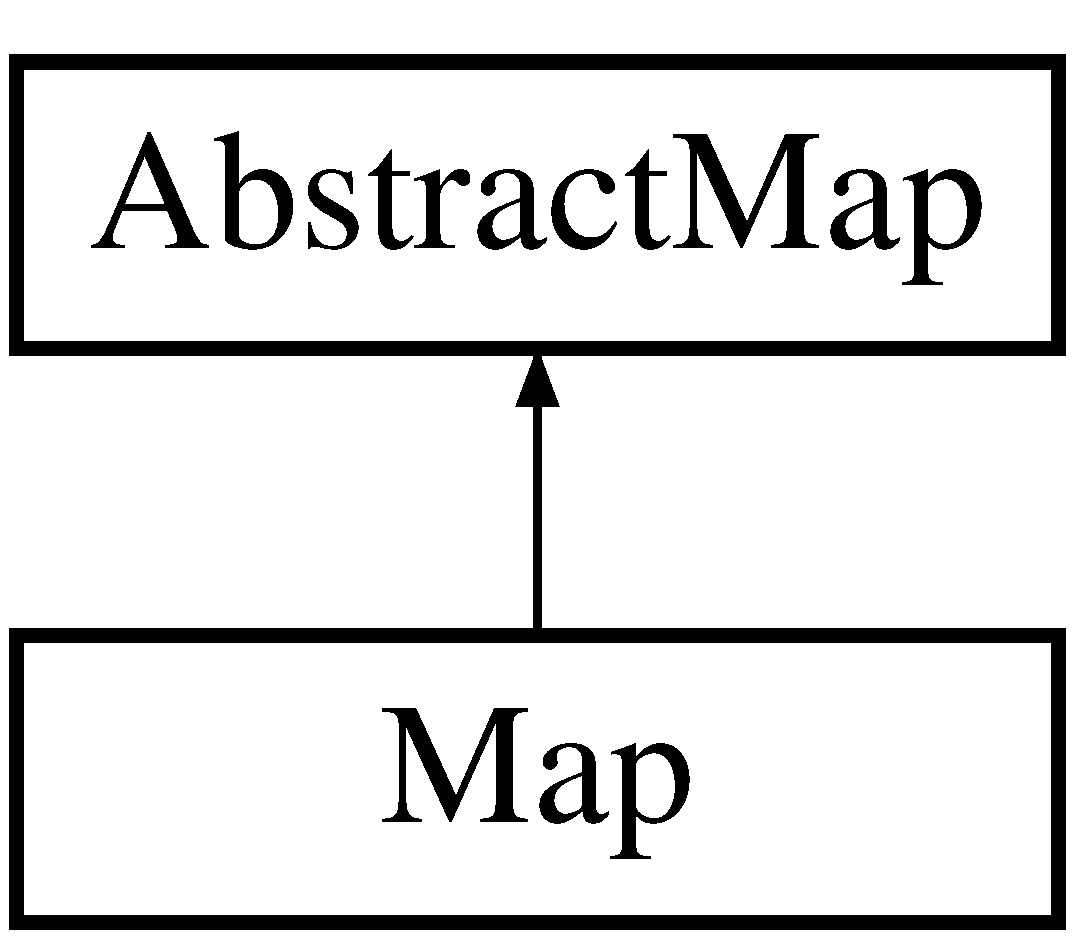
\includegraphics[height=2.000000cm]{class_abstract_map}
\end{center}
\end{figure}
\subsection*{Public Member Functions}
\begin{DoxyCompactItemize}
\item 
\mbox{\Hypertarget{class_abstract_map_ab2fbb46108e2905fb1193a67510d41f0}\label{class_abstract_map_ab2fbb46108e2905fb1193a67510d41f0}} 
virtual \hyperlink{class_abstract_map_ab2fbb46108e2905fb1193a67510d41f0}{$\sim$\+Abstract\+Map} ()
\begin{DoxyCompactList}\small\item\em Virtual Destructor. \end{DoxyCompactList}\item 
virtual void \hyperlink{class_abstract_map_a9938512c5ef94370786a3d1a72aa7e37}{add\+City} (\hyperlink{class_city}{City} $\ast$)=0
\begin{DoxyCompactList}\small\item\em Adds the provided city to this map. \end{DoxyCompactList}\item 
virtual bool \hyperlink{class_abstract_map_a179d25c28087d9090314caff024b1f46}{add\+Street} (\hyperlink{class_street}{Street} $\ast$)=0
\begin{DoxyCompactList}\small\item\em Adds the provided street to this map. If the cities linked by the street have not been added to this map before, the street is not added. \end{DoxyCompactList}\item 
virtual \hyperlink{class_city}{City} $\ast$ \hyperlink{class_abstract_map_abda0a780cdd294491b1dff5c088b96a2}{find\+\_\+city} (const Q\+String city\+\_\+name) const =0
\begin{DoxyCompactList}\small\item\em Search for a city in this map by given name. \end{DoxyCompactList}\item 
virtual std\+::vector$<$ \hyperlink{class_street}{Street} $\ast$ $>$ \hyperlink{class_abstract_map_a228d43b47211f3836fdc66760831d61d}{get\+\_\+street\+\_\+list} (const \hyperlink{class_city}{City} $\ast$city) const =0
\begin{DoxyCompactList}\small\item\em Search for streets in this map. \end{DoxyCompactList}\item 
virtual \hyperlink{class_city}{City} $\ast$ \hyperlink{class_abstract_map_ab372998d6ab42b67d1fd7b97b2c380f2}{get\+\_\+opposite\+\_\+city} (const \hyperlink{class_street}{Street} $\ast$street, const \hyperlink{class_city}{City} $\ast$city) const =0
\begin{DoxyCompactList}\small\item\em Look for opposite city. \end{DoxyCompactList}\item 
virtual double \hyperlink{class_abstract_map_a19a4ead06c11b297f7ec9731574fa326}{get\+\_\+length} (const \hyperlink{class_street}{Street} $\ast$street) const =0
\begin{DoxyCompactList}\small\item\em Calculate the street length. \end{DoxyCompactList}\end{DoxyCompactItemize}


\subsection{Member Function Documentation}
\mbox{\Hypertarget{class_abstract_map_a9938512c5ef94370786a3d1a72aa7e37}\label{class_abstract_map_a9938512c5ef94370786a3d1a72aa7e37}} 
\index{Abstract\+Map@{Abstract\+Map}!add\+City@{add\+City}}
\index{add\+City@{add\+City}!Abstract\+Map@{Abstract\+Map}}
\subsubsection{\texorpdfstring{add\+City()}{addCity()}}
{\footnotesize\ttfamily virtual void Abstract\+Map\+::add\+City (\begin{DoxyParamCaption}\item[{\hyperlink{class_city}{City} $\ast$}]{ }\end{DoxyParamCaption})\hspace{0.3cm}{\ttfamily [pure virtual]}}



Adds the provided city to this map. 


\begin{DoxyParams}{Parameters}
{\em Pointer} & to city to be added \\
\hline
\end{DoxyParams}
\begin{DoxyReturn}{Returns}
true if the has been added 
\end{DoxyReturn}


Implemented in \hyperlink{class_map_a3313ee9e1dc1bc7e8865ab2c64082ca8}{Map}.

\mbox{\Hypertarget{class_abstract_map_a179d25c28087d9090314caff024b1f46}\label{class_abstract_map_a179d25c28087d9090314caff024b1f46}} 
\index{Abstract\+Map@{Abstract\+Map}!add\+Street@{add\+Street}}
\index{add\+Street@{add\+Street}!Abstract\+Map@{Abstract\+Map}}
\subsubsection{\texorpdfstring{add\+Street()}{addStreet()}}
{\footnotesize\ttfamily virtual bool Abstract\+Map\+::add\+Street (\begin{DoxyParamCaption}\item[{\hyperlink{class_street}{Street} $\ast$}]{ }\end{DoxyParamCaption})\hspace{0.3cm}{\ttfamily [pure virtual]}}



Adds the provided street to this map. If the cities linked by the street have not been added to this map before, the street is not added. 


\begin{DoxyParams}{Parameters}
{\em Pointer} & to the street to be added \\
\hline
\end{DoxyParams}
\begin{DoxyReturn}{Returns}
true if the street has beed added. 
\end{DoxyReturn}


Implemented in \hyperlink{class_map_a9e5ad7aea193a11e3a5e2f0bb045e818}{Map}.

\mbox{\Hypertarget{class_abstract_map_abda0a780cdd294491b1dff5c088b96a2}\label{class_abstract_map_abda0a780cdd294491b1dff5c088b96a2}} 
\index{Abstract\+Map@{Abstract\+Map}!find\+\_\+city@{find\+\_\+city}}
\index{find\+\_\+city@{find\+\_\+city}!Abstract\+Map@{Abstract\+Map}}
\subsubsection{\texorpdfstring{find\+\_\+city()}{find\_city()}}
{\footnotesize\ttfamily virtual \hyperlink{class_city}{City}$\ast$ Abstract\+Map\+::find\+\_\+city (\begin{DoxyParamCaption}\item[{const Q\+String}]{city\+\_\+name }\end{DoxyParamCaption}) const\hspace{0.3cm}{\ttfamily [pure virtual]}}



Search for a city in this map by given name. 


\begin{DoxyParams}{Parameters}
{\em name} & \\
\hline
\end{DoxyParams}
\begin{DoxyReturn}{Returns}
the city pointer, if city not found N\+U\+LL 
\end{DoxyReturn}


Implemented in \hyperlink{class_map_acb7d6869cfe4e6e91d3a1c5155ad89b2}{Map}.

\mbox{\Hypertarget{class_abstract_map_a19a4ead06c11b297f7ec9731574fa326}\label{class_abstract_map_a19a4ead06c11b297f7ec9731574fa326}} 
\index{Abstract\+Map@{Abstract\+Map}!get\+\_\+length@{get\+\_\+length}}
\index{get\+\_\+length@{get\+\_\+length}!Abstract\+Map@{Abstract\+Map}}
\subsubsection{\texorpdfstring{get\+\_\+length()}{get\_length()}}
{\footnotesize\ttfamily virtual double Abstract\+Map\+::get\+\_\+length (\begin{DoxyParamCaption}\item[{const \hyperlink{class_street}{Street} $\ast$}]{street }\end{DoxyParamCaption}) const\hspace{0.3cm}{\ttfamily [pure virtual]}}



Calculate the street length. 


\begin{DoxyParams}{Parameters}
{\em street} & \\
\hline
\end{DoxyParams}
\begin{DoxyReturn}{Returns}
length of the street 
\end{DoxyReturn}


Implemented in \hyperlink{class_map_a041fd9e53a2e80a0fb3b1e11e3fdf1e9}{Map}.

\mbox{\Hypertarget{class_abstract_map_ab372998d6ab42b67d1fd7b97b2c380f2}\label{class_abstract_map_ab372998d6ab42b67d1fd7b97b2c380f2}} 
\index{Abstract\+Map@{Abstract\+Map}!get\+\_\+opposite\+\_\+city@{get\+\_\+opposite\+\_\+city}}
\index{get\+\_\+opposite\+\_\+city@{get\+\_\+opposite\+\_\+city}!Abstract\+Map@{Abstract\+Map}}
\subsubsection{\texorpdfstring{get\+\_\+opposite\+\_\+city()}{get\_opposite\_city()}}
{\footnotesize\ttfamily virtual \hyperlink{class_city}{City}$\ast$ Abstract\+Map\+::get\+\_\+opposite\+\_\+city (\begin{DoxyParamCaption}\item[{const \hyperlink{class_street}{Street} $\ast$}]{street,  }\item[{const \hyperlink{class_city}{City} $\ast$}]{city }\end{DoxyParamCaption}) const\hspace{0.3cm}{\ttfamily [pure virtual]}}



Look for opposite city. 


\begin{DoxyParams}{Parameters}
{\em street} & \\
\hline
{\em city} & \\
\hline
\end{DoxyParams}
\begin{DoxyReturn}{Returns}
opposite city of the street. If city has no connection to street returns N\+U\+LL. 
\end{DoxyReturn}


Implemented in \hyperlink{class_map_ac52744dc6f969ca6cdbca96f89d314ed}{Map}.

\mbox{\Hypertarget{class_abstract_map_a228d43b47211f3836fdc66760831d61d}\label{class_abstract_map_a228d43b47211f3836fdc66760831d61d}} 
\index{Abstract\+Map@{Abstract\+Map}!get\+\_\+street\+\_\+list@{get\+\_\+street\+\_\+list}}
\index{get\+\_\+street\+\_\+list@{get\+\_\+street\+\_\+list}!Abstract\+Map@{Abstract\+Map}}
\subsubsection{\texorpdfstring{get\+\_\+street\+\_\+list()}{get\_street\_list()}}
{\footnotesize\ttfamily virtual std\+::vector$<$\hyperlink{class_street}{Street}$\ast$$>$ Abstract\+Map\+::get\+\_\+street\+\_\+list (\begin{DoxyParamCaption}\item[{const \hyperlink{class_city}{City} $\ast$}]{city }\end{DoxyParamCaption}) const\hspace{0.3cm}{\ttfamily [pure virtual]}}



Search for streets in this map. 


\begin{DoxyParams}{Parameters}
{\em city} & where you want the street\+\_\+list from \\
\hline
\end{DoxyParams}
\begin{DoxyReturn}{Returns}
a list of all streets in this map connected to provided city. 
\end{DoxyReturn}


Implemented in \hyperlink{class_map_a24c8fa29273d26e301f889ab81d696e3}{Map}.



The documentation for this class was generated from the following files\+:\begin{DoxyCompactItemize}
\item 
abstractmap.\+h\item 
abstractmap.\+cpp\end{DoxyCompactItemize}

\hypertarget{class_add_street_dialog}{}\section{Add\+Street\+Dialog Class Reference}
\label{class_add_street_dialog}\index{Add\+Street\+Dialog@{Add\+Street\+Dialog}}
Inheritance diagram for Add\+Street\+Dialog\+:\begin{figure}[H]
\begin{center}
\leavevmode
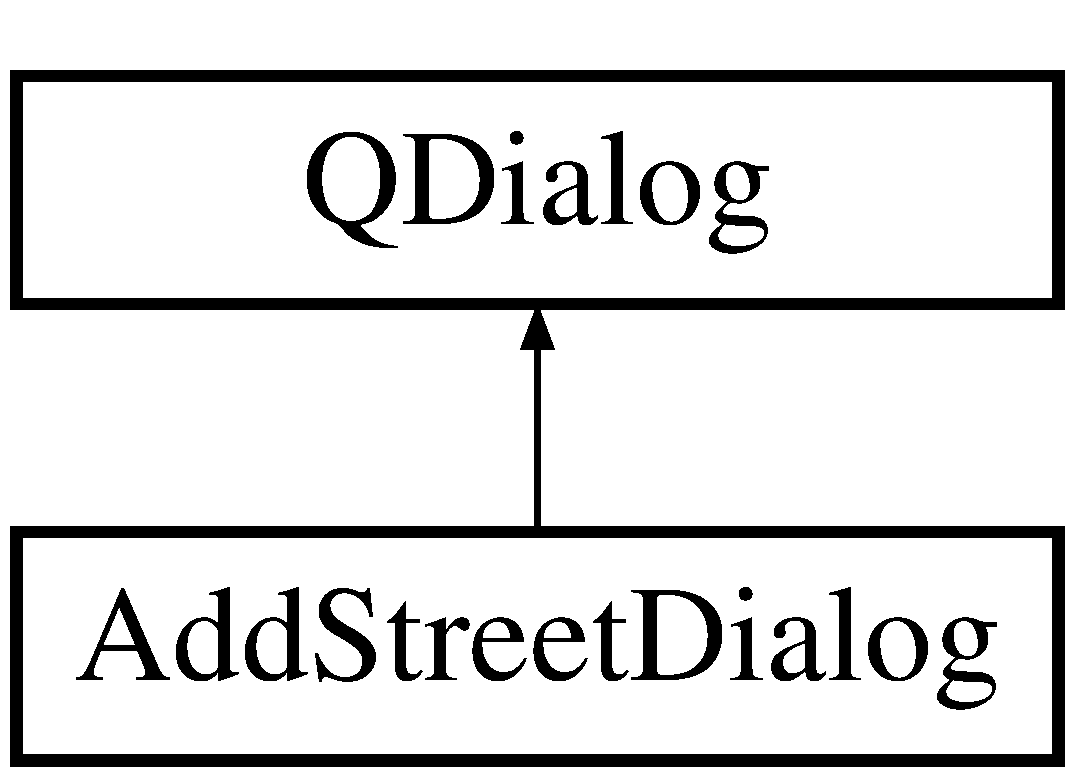
\includegraphics[height=2.000000cm]{class_add_street_dialog}
\end{center}
\end{figure}
\subsection*{Public Member Functions}
\begin{DoxyCompactItemize}
\item 
\mbox{\Hypertarget{class_add_street_dialog_a82f4a0eaa9a88d7a6701d711085a3a58}\label{class_add_street_dialog_a82f4a0eaa9a88d7a6701d711085a3a58}} 
{\bfseries Add\+Street\+Dialog} (Q\+Widget $\ast$parent=0)
\item 
void \hyperlink{class_add_street_dialog_a78dbf0fdb7a3f345ceabaf14b0439fd1}{add\+City\+Name} (Q\+String name)
\begin{DoxyCompactList}\small\item\em Adds a name to the two city comboboxes. \end{DoxyCompactList}\item 
Q\+String \hyperlink{class_add_street_dialog_a180380683de12d32099d9aacf19673ae}{get\+City1\+Name} ()
\begin{DoxyCompactList}\small\item\em Returns the name of city 1. \end{DoxyCompactList}\item 
Q\+String \hyperlink{class_add_street_dialog_a119252f87220d48c4a49d64a96c0f5fd}{get\+City2\+Name} ()
\begin{DoxyCompactList}\small\item\em Returns the name of city 2. \end{DoxyCompactList}\end{DoxyCompactItemize}


\subsection{Member Function Documentation}
\mbox{\Hypertarget{class_add_street_dialog_a78dbf0fdb7a3f345ceabaf14b0439fd1}\label{class_add_street_dialog_a78dbf0fdb7a3f345ceabaf14b0439fd1}} 
\index{Add\+Street\+Dialog@{Add\+Street\+Dialog}!add\+City\+Name@{add\+City\+Name}}
\index{add\+City\+Name@{add\+City\+Name}!Add\+Street\+Dialog@{Add\+Street\+Dialog}}
\subsubsection{\texorpdfstring{add\+City\+Name()}{addCityName()}}
{\footnotesize\ttfamily void Add\+Street\+Dialog\+::add\+City\+Name (\begin{DoxyParamCaption}\item[{Q\+String}]{name }\end{DoxyParamCaption})}



Adds a name to the two city comboboxes. 


\begin{DoxyParams}{Parameters}
{\em name} & the name to be added \\
\hline
\end{DoxyParams}
\mbox{\Hypertarget{class_add_street_dialog_a180380683de12d32099d9aacf19673ae}\label{class_add_street_dialog_a180380683de12d32099d9aacf19673ae}} 
\index{Add\+Street\+Dialog@{Add\+Street\+Dialog}!get\+City1\+Name@{get\+City1\+Name}}
\index{get\+City1\+Name@{get\+City1\+Name}!Add\+Street\+Dialog@{Add\+Street\+Dialog}}
\subsubsection{\texorpdfstring{get\+City1\+Name()}{getCity1Name()}}
{\footnotesize\ttfamily Q\+String Add\+Street\+Dialog\+::get\+City1\+Name (\begin{DoxyParamCaption}{ }\end{DoxyParamCaption})}



Returns the name of city 1. 

\begin{DoxyReturn}{Returns}
name of city 1 
\end{DoxyReturn}
\mbox{\Hypertarget{class_add_street_dialog_a119252f87220d48c4a49d64a96c0f5fd}\label{class_add_street_dialog_a119252f87220d48c4a49d64a96c0f5fd}} 
\index{Add\+Street\+Dialog@{Add\+Street\+Dialog}!get\+City2\+Name@{get\+City2\+Name}}
\index{get\+City2\+Name@{get\+City2\+Name}!Add\+Street\+Dialog@{Add\+Street\+Dialog}}
\subsubsection{\texorpdfstring{get\+City2\+Name()}{getCity2Name()}}
{\footnotesize\ttfamily Q\+String Add\+Street\+Dialog\+::get\+City2\+Name (\begin{DoxyParamCaption}{ }\end{DoxyParamCaption})}



Returns the name of city 2. 

\begin{DoxyReturn}{Returns}
name of city 2 
\end{DoxyReturn}


The documentation for this class was generated from the following files\+:\begin{DoxyCompactItemize}
\item 
addstreetdialog.\+h\item 
addstreetdialog.\+cpp\end{DoxyCompactItemize}

\hypertarget{class_city}{}\section{City Class Reference}
\label{class_city}\index{City@{City}}
\subsection*{Public Member Functions}
\begin{DoxyCompactItemize}
\item 
\hyperlink{class_city_a9e29f32d33f56bdf59cba425a7e08bd8}{City} (Q\+String name, int x, int y)
\begin{DoxyCompactList}\small\item\em Constructor for the class \hyperlink{class_city}{City}. \end{DoxyCompactList}\item 
void \hyperlink{class_city_a3d22cac343c40bf53d6bc8d831ac4262}{draw} (Q\+Graphics\+Scene \&scene)
\begin{DoxyCompactList}\small\item\em Draws this city on a given Q\+Graphics\+Scene. \end{DoxyCompactList}\item 
int \hyperlink{class_city_a31a58c2f36a488519ce6bb8373e6a329}{getX} ()
\begin{DoxyCompactList}\small\item\em Returns the x-\/position of this city. \end{DoxyCompactList}\item 
int \hyperlink{class_city_ada68b2e07e01a526b68011c3a638ee96}{getY} ()
\begin{DoxyCompactList}\small\item\em Returns the y-\/position of this city. \end{DoxyCompactList}\item 
Q\+String \hyperlink{class_city_afe733410d61155d8a4013293b0b72408}{get\+Name} ()
\begin{DoxyCompactList}\small\item\em Returns the name of this city. \end{DoxyCompactList}\end{DoxyCompactItemize}


\subsection{Constructor \& Destructor Documentation}
\mbox{\Hypertarget{class_city_a9e29f32d33f56bdf59cba425a7e08bd8}\label{class_city_a9e29f32d33f56bdf59cba425a7e08bd8}} 
\index{City@{City}!City@{City}}
\index{City@{City}!City@{City}}
\subsubsection{\texorpdfstring{City()}{City()}}
{\footnotesize\ttfamily City\+::\+City (\begin{DoxyParamCaption}\item[{Q\+String}]{name,  }\item[{int}]{x,  }\item[{int}]{y }\end{DoxyParamCaption})}



Constructor for the class \hyperlink{class_city}{City}. 


\begin{DoxyParams}{Parameters}
{\em name} & The name of the \hyperlink{class_city}{City} \\
\hline
{\em x} & x-\/position of the \hyperlink{class_city}{City} \\
\hline
{\em y} & y-\/position of the \hyperlink{class_city}{City} \\
\hline
\end{DoxyParams}


\subsection{Member Function Documentation}
\mbox{\Hypertarget{class_city_a3d22cac343c40bf53d6bc8d831ac4262}\label{class_city_a3d22cac343c40bf53d6bc8d831ac4262}} 
\index{City@{City}!draw@{draw}}
\index{draw@{draw}!City@{City}}
\subsubsection{\texorpdfstring{draw()}{draw()}}
{\footnotesize\ttfamily void City\+::draw (\begin{DoxyParamCaption}\item[{Q\+Graphics\+Scene \&}]{scene }\end{DoxyParamCaption})}



Draws this city on a given Q\+Graphics\+Scene. 


\begin{DoxyParams}{Parameters}
{\em Q\+Graphics\+Scene} & scene \\
\hline
\end{DoxyParams}
\mbox{\Hypertarget{class_city_afe733410d61155d8a4013293b0b72408}\label{class_city_afe733410d61155d8a4013293b0b72408}} 
\index{City@{City}!get\+Name@{get\+Name}}
\index{get\+Name@{get\+Name}!City@{City}}
\subsubsection{\texorpdfstring{get\+Name()}{getName()}}
{\footnotesize\ttfamily Q\+String City\+::get\+Name (\begin{DoxyParamCaption}{ }\end{DoxyParamCaption})}



Returns the name of this city. 

\begin{DoxyReturn}{Returns}
Q\+String name 
\end{DoxyReturn}
\mbox{\Hypertarget{class_city_a31a58c2f36a488519ce6bb8373e6a329}\label{class_city_a31a58c2f36a488519ce6bb8373e6a329}} 
\index{City@{City}!getX@{getX}}
\index{getX@{getX}!City@{City}}
\subsubsection{\texorpdfstring{get\+X()}{getX()}}
{\footnotesize\ttfamily int City\+::getX (\begin{DoxyParamCaption}{ }\end{DoxyParamCaption})}



Returns the x-\/position of this city. 

\begin{DoxyReturn}{Returns}
x-\/position 
\end{DoxyReturn}
\mbox{\Hypertarget{class_city_ada68b2e07e01a526b68011c3a638ee96}\label{class_city_ada68b2e07e01a526b68011c3a638ee96}} 
\index{City@{City}!getY@{getY}}
\index{getY@{getY}!City@{City}}
\subsubsection{\texorpdfstring{get\+Y()}{getY()}}
{\footnotesize\ttfamily int City\+::getY (\begin{DoxyParamCaption}{ }\end{DoxyParamCaption})}



Returns the y-\/position of this city. 

\begin{DoxyReturn}{Returns}
y-\/position 
\end{DoxyReturn}


The documentation for this class was generated from the following files\+:\begin{DoxyCompactItemize}
\item 
city.\+h\item 
city.\+cpp\end{DoxyCompactItemize}

\hypertarget{class_dijkstra}{}\section{Dijkstra Class Reference}
\label{class_dijkstra}\index{Dijkstra@{Dijkstra}}
\subsection*{Static Public Member Functions}
\begin{DoxyCompactItemize}
\item 
static std\+::vector$<$ \hyperlink{class_street}{Street} $\ast$ $>$ \hyperlink{class_dijkstra_aa9c3cc0e47ab3a865dbe9f4e152af71f}{search} (const \hyperlink{class_abstract_map}{Abstract\+Map} \&map, Q\+String start, Q\+String target)
\begin{DoxyCompactList}\small\item\em \hyperlink{class_dijkstra}{Dijkstra} Algorithm to find the shortest path between two towns. \end{DoxyCompactList}\item 
\mbox{\Hypertarget{class_dijkstra_aa6c60bc89d86bf877cc586557ae8f564}\label{class_dijkstra_aa6c60bc89d86bf877cc586557ae8f564}} 
static void {\bfseries draw\+Way} (std\+::vector$<$ \hyperlink{class_street}{Street} $\ast$$>$ \&way, Q\+Graphics\+Scene \&scene)
\end{DoxyCompactItemize}


\subsection{Member Function Documentation}
\mbox{\Hypertarget{class_dijkstra_aa9c3cc0e47ab3a865dbe9f4e152af71f}\label{class_dijkstra_aa9c3cc0e47ab3a865dbe9f4e152af71f}} 
\index{Dijkstra@{Dijkstra}!search@{search}}
\index{search@{search}!Dijkstra@{Dijkstra}}
\subsubsection{\texorpdfstring{search()}{search()}}
{\footnotesize\ttfamily std\+::vector$<$ \hyperlink{class_street}{Street} $\ast$ $>$ Dijkstra\+::search (\begin{DoxyParamCaption}\item[{const \hyperlink{class_abstract_map}{Abstract\+Map} \&}]{map,  }\item[{Q\+String}]{start,  }\item[{Q\+String}]{target }\end{DoxyParamCaption})\hspace{0.3cm}{\ttfamily [static]}}



\hyperlink{class_dijkstra}{Dijkstra} Algorithm to find the shortest path between two towns. 


\begin{DoxyParams}{Parameters}
{\em start} & Name of the start town. \\
\hline
{\em target} & Name of the target town.\\
\hline
\end{DoxyParams}
\begin{DoxyReturn}{Returns}
Pointer to a list of streets between the towns. Empty list if no connection found. 
\end{DoxyReturn}


The documentation for this class was generated from the following files\+:\begin{DoxyCompactItemize}
\item 
dijkstra.\+h\item 
dijkstra.\+cpp\end{DoxyCompactItemize}

\hypertarget{class_dijkstra_dialog}{}\section{Dijkstra\+Dialog Class Reference}
\label{class_dijkstra_dialog}\index{Dijkstra\+Dialog@{Dijkstra\+Dialog}}
Inheritance diagram for Dijkstra\+Dialog\+:\begin{figure}[H]
\begin{center}
\leavevmode
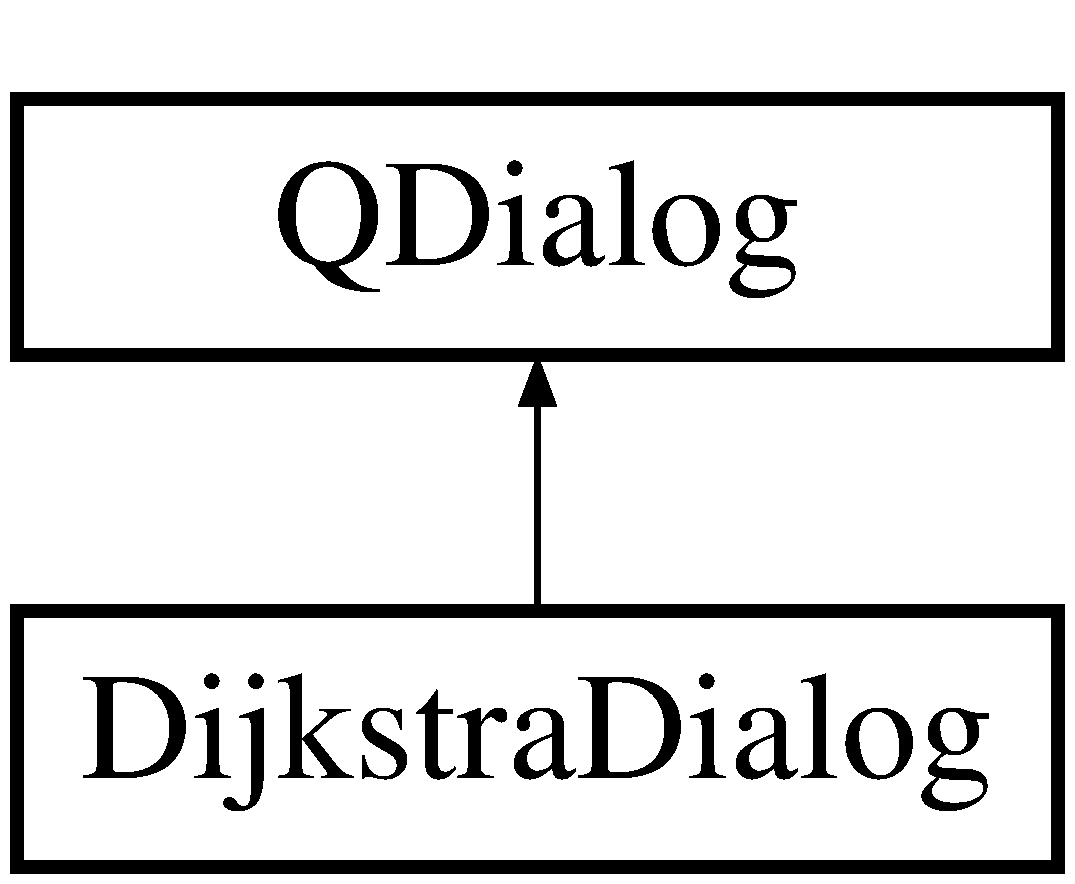
\includegraphics[height=2.000000cm]{class_dijkstra_dialog}
\end{center}
\end{figure}
\subsection*{Public Member Functions}
\begin{DoxyCompactItemize}
\item 
\mbox{\Hypertarget{class_dijkstra_dialog_a507b5273e2491adfe5d070a7f989ad3c}\label{class_dijkstra_dialog_a507b5273e2491adfe5d070a7f989ad3c}} 
{\bfseries Dijkstra\+Dialog} (Q\+Widget $\ast$parent=0)
\item 
void \hyperlink{class_dijkstra_dialog_ae4bd48d8dc7d10e4cda0e8638bb1d22e}{start\+Dijkstra} (Q\+Graphics\+Scene \&scene, \hyperlink{class_map}{Map} \&map)
\begin{DoxyCompactList}\small\item\em Starts the dijkstra algo and draws the way. \end{DoxyCompactList}\item 
void \hyperlink{class_dijkstra_dialog_ae4d6de8a537996c265140d3415acd031}{add\+City\+Name} (Q\+String name)
\begin{DoxyCompactList}\small\item\em Adds a name to city comboboxes. \end{DoxyCompactList}\end{DoxyCompactItemize}


\subsection{Member Function Documentation}
\mbox{\Hypertarget{class_dijkstra_dialog_ae4d6de8a537996c265140d3415acd031}\label{class_dijkstra_dialog_ae4d6de8a537996c265140d3415acd031}} 
\index{Dijkstra\+Dialog@{Dijkstra\+Dialog}!add\+City\+Name@{add\+City\+Name}}
\index{add\+City\+Name@{add\+City\+Name}!Dijkstra\+Dialog@{Dijkstra\+Dialog}}
\subsubsection{\texorpdfstring{add\+City\+Name()}{addCityName()}}
{\footnotesize\ttfamily void Dijkstra\+Dialog\+::add\+City\+Name (\begin{DoxyParamCaption}\item[{Q\+String}]{name }\end{DoxyParamCaption})}



Adds a name to city comboboxes. 


\begin{DoxyParams}{Parameters}
{\em name} & \\
\hline
\end{DoxyParams}
\mbox{\Hypertarget{class_dijkstra_dialog_ae4bd48d8dc7d10e4cda0e8638bb1d22e}\label{class_dijkstra_dialog_ae4bd48d8dc7d10e4cda0e8638bb1d22e}} 
\index{Dijkstra\+Dialog@{Dijkstra\+Dialog}!start\+Dijkstra@{start\+Dijkstra}}
\index{start\+Dijkstra@{start\+Dijkstra}!Dijkstra\+Dialog@{Dijkstra\+Dialog}}
\subsubsection{\texorpdfstring{start\+Dijkstra()}{startDijkstra()}}
{\footnotesize\ttfamily void Dijkstra\+Dialog\+::start\+Dijkstra (\begin{DoxyParamCaption}\item[{Q\+Graphics\+Scene \&}]{scene,  }\item[{\hyperlink{class_map}{Map} \&}]{map }\end{DoxyParamCaption})}



Starts the dijkstra algo and draws the way. 


\begin{DoxyParams}{Parameters}
{\em scene} & this scnene will be used to draw the way on Q\+Graphicsscene \\
\hline
{\em map} & the map with the streets for the dijkstra algo \\
\hline
\end{DoxyParams}


The documentation for this class was generated from the following files\+:\begin{DoxyCompactItemize}
\item 
dijkstradialog.\+h\item 
dijkstradialog.\+cpp\end{DoxyCompactItemize}

\hypertarget{class_main_window}{}\section{Main\+Window Class Reference}
\label{class_main_window}\index{Main\+Window@{Main\+Window}}
Inheritance diagram for Main\+Window\+:\begin{figure}[H]
\begin{center}
\leavevmode
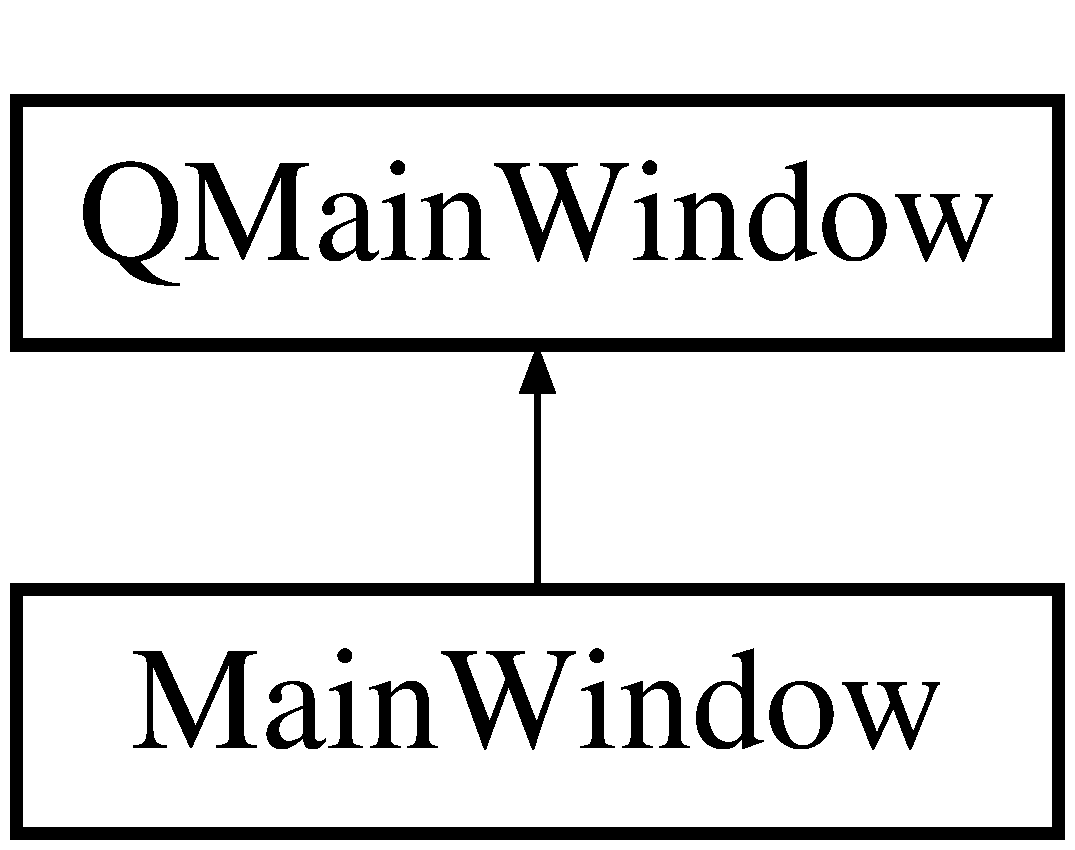
\includegraphics[height=2.000000cm]{class_main_window}
\end{center}
\end{figure}
\subsection*{Public Member Functions}
\begin{DoxyCompactItemize}
\item 
\mbox{\Hypertarget{class_main_window_a8b244be8b7b7db1b08de2a2acb9409db}\label{class_main_window_a8b244be8b7b7db1b08de2a2acb9409db}} 
{\bfseries Main\+Window} (Q\+Widget $\ast$parent=0)
\end{DoxyCompactItemize}


The documentation for this class was generated from the following files\+:\begin{DoxyCompactItemize}
\item 
mainwindow.\+h\item 
mainwindow.\+cpp\end{DoxyCompactItemize}

\hypertarget{class_map}{}\section{Map Class Reference}
\label{class_map}\index{Map@{Map}}
Inheritance diagram for Map\+:\begin{figure}[H]
\begin{center}
\leavevmode
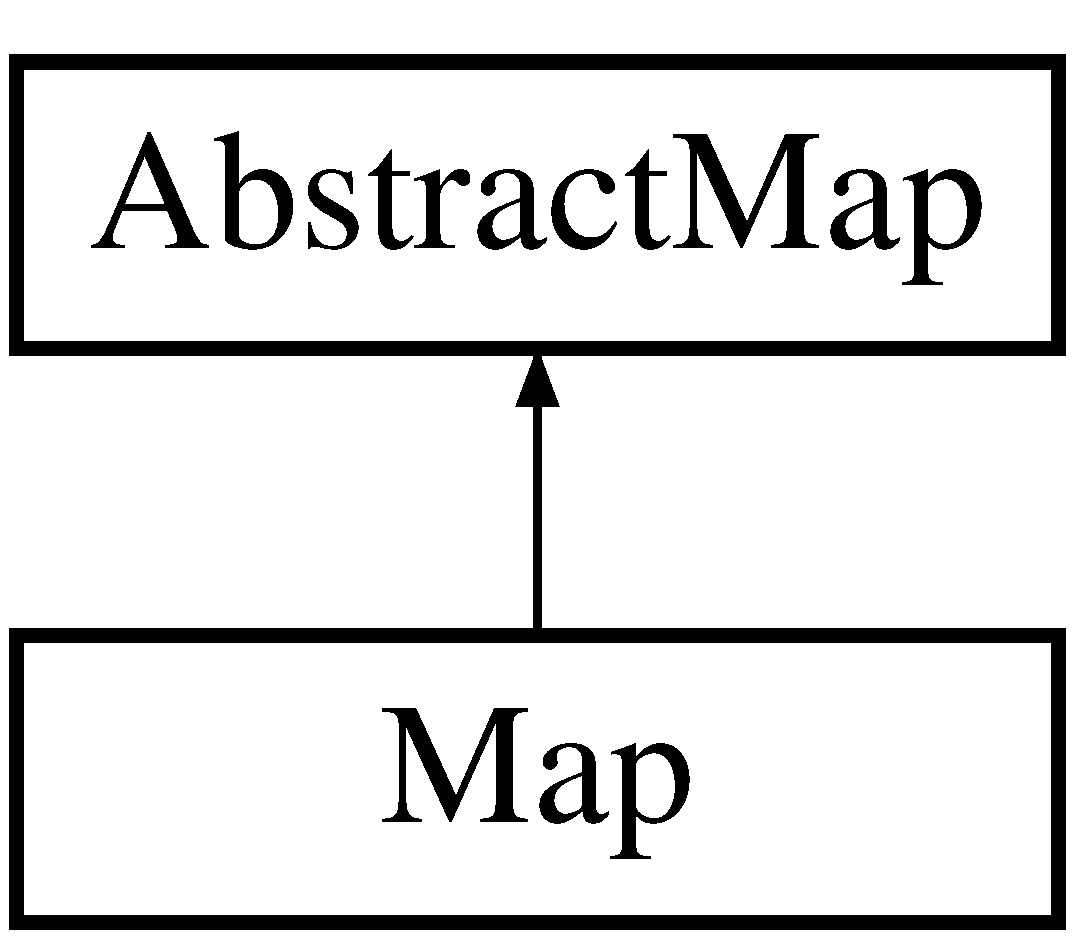
\includegraphics[height=2.000000cm]{class_map}
\end{center}
\end{figure}
\subsection*{Public Member Functions}
\begin{DoxyCompactItemize}
\item 
void \hyperlink{class_map_a3313ee9e1dc1bc7e8865ab2c64082ca8}{add\+City} (\hyperlink{class_city}{City} $\ast$city)
\begin{DoxyCompactList}\small\item\em Adds a city to the map. \end{DoxyCompactList}\item 
std\+::vector$<$ \hyperlink{class_city}{City} $\ast$ $>$ \hyperlink{class_map_aac96173f49b430365521708440055772}{get\+Cities} ()
\begin{DoxyCompactList}\small\item\em Returns a list conataining the pointers to all cities on this map. \end{DoxyCompactList}\item 
bool \hyperlink{class_map_a9e5ad7aea193a11e3a5e2f0bb045e818}{add\+Street} (\hyperlink{class_street}{Street} $\ast$street)
\begin{DoxyCompactList}\small\item\em Adds a street to the map if it isn\textquotesingle{}t on there. \end{DoxyCompactList}\item 
void \hyperlink{class_map_af7386ac56bf2ff2d5598ae6e08dc8193}{draw} (Q\+Graphics\+Scene \&scene)
\begin{DoxyCompactList}\small\item\em Draws the whole map onto a given Q\+Graphicsscene. \end{DoxyCompactList}\item 
virtual \hyperlink{class_city}{City} $\ast$ \hyperlink{class_map_acb7d6869cfe4e6e91d3a1c5155ad89b2}{find\+\_\+city} (const Q\+String city\+\_\+name) const
\begin{DoxyCompactList}\small\item\em Finds a city with the specified name. \end{DoxyCompactList}\item 
virtual std\+::vector$<$ \hyperlink{class_street}{Street} $\ast$ $>$ \hyperlink{class_map_a24c8fa29273d26e301f889ab81d696e3}{get\+\_\+street\+\_\+list} (const \hyperlink{class_city}{City} $\ast$city) const
\begin{DoxyCompactList}\small\item\em Search for all streets connected to the given city. \end{DoxyCompactList}\item 
virtual \hyperlink{class_city}{City} $\ast$ \hyperlink{class_map_ac52744dc6f969ca6cdbca96f89d314ed}{get\+\_\+opposite\+\_\+city} (const \hyperlink{class_street}{Street} $\ast$street, const \hyperlink{class_city}{City} $\ast$city) const
\begin{DoxyCompactList}\small\item\em Look for the city being at the other end of a given street. \end{DoxyCompactList}\item 
virtual double \hyperlink{class_map_a041fd9e53a2e80a0fb3b1e11e3fdf1e9}{get\+\_\+length} (const \hyperlink{class_street}{Street} $\ast$street) const
\begin{DoxyCompactList}\small\item\em Calculates the length of a street. \end{DoxyCompactList}\end{DoxyCompactItemize}


\subsection{Member Function Documentation}
\mbox{\Hypertarget{class_map_a3313ee9e1dc1bc7e8865ab2c64082ca8}\label{class_map_a3313ee9e1dc1bc7e8865ab2c64082ca8}} 
\index{Map@{Map}!add\+City@{add\+City}}
\index{add\+City@{add\+City}!Map@{Map}}
\subsubsection{\texorpdfstring{add\+City()}{addCity()}}
{\footnotesize\ttfamily void Map\+::add\+City (\begin{DoxyParamCaption}\item[{\hyperlink{class_city}{City} $\ast$}]{city }\end{DoxyParamCaption})\hspace{0.3cm}{\ttfamily [virtual]}}



Adds a city to the map. 

The class map contains a list (a vector) of cities. If the map doesn\textquotesingle{}t already contain the given city, this function adds it to the list.


\begin{DoxyParams}{Parameters}
{\em The} & city to be added \\
\hline
\end{DoxyParams}


Implements \hyperlink{class_abstract_map_a9938512c5ef94370786a3d1a72aa7e37}{Abstract\+Map}.

\mbox{\Hypertarget{class_map_a9e5ad7aea193a11e3a5e2f0bb045e818}\label{class_map_a9e5ad7aea193a11e3a5e2f0bb045e818}} 
\index{Map@{Map}!add\+Street@{add\+Street}}
\index{add\+Street@{add\+Street}!Map@{Map}}
\subsubsection{\texorpdfstring{add\+Street()}{addStreet()}}
{\footnotesize\ttfamily bool Map\+::add\+Street (\begin{DoxyParamCaption}\item[{\hyperlink{class_street}{Street} $\ast$}]{street }\end{DoxyParamCaption})\hspace{0.3cm}{\ttfamily [virtual]}}



Adds a street to the map if it isn\textquotesingle{}t on there. 


\begin{DoxyParams}{Parameters}
{\em The} & street to be added \\
\hline
\end{DoxyParams}
\begin{DoxyReturn}{Returns}
false if the street cant be added 
\end{DoxyReturn}


Implements \hyperlink{class_abstract_map_a179d25c28087d9090314caff024b1f46}{Abstract\+Map}.

\mbox{\Hypertarget{class_map_af7386ac56bf2ff2d5598ae6e08dc8193}\label{class_map_af7386ac56bf2ff2d5598ae6e08dc8193}} 
\index{Map@{Map}!draw@{draw}}
\index{draw@{draw}!Map@{Map}}
\subsubsection{\texorpdfstring{draw()}{draw()}}
{\footnotesize\ttfamily void Map\+::draw (\begin{DoxyParamCaption}\item[{Q\+Graphics\+Scene \&}]{scene }\end{DoxyParamCaption})}



Draws the whole map onto a given Q\+Graphicsscene. 


\begin{DoxyParams}{Parameters}
{\em scene} & The scene to draw on \\
\hline
\end{DoxyParams}
\mbox{\Hypertarget{class_map_acb7d6869cfe4e6e91d3a1c5155ad89b2}\label{class_map_acb7d6869cfe4e6e91d3a1c5155ad89b2}} 
\index{Map@{Map}!find\+\_\+city@{find\+\_\+city}}
\index{find\+\_\+city@{find\+\_\+city}!Map@{Map}}
\subsubsection{\texorpdfstring{find\+\_\+city()}{find\_city()}}
{\footnotesize\ttfamily \hyperlink{class_city}{City} $\ast$ Map\+::find\+\_\+city (\begin{DoxyParamCaption}\item[{const Q\+String}]{city\+\_\+name }\end{DoxyParamCaption}) const\hspace{0.3cm}{\ttfamily [virtual]}}



Finds a city with the specified name. 


\begin{DoxyParams}{Parameters}
{\em city\+\_\+name} & The name of the city to be found \\
\hline
\end{DoxyParams}
\begin{DoxyReturn}{Returns}
A pointer to the city / N\+U\+LL (if it isn\textquotesingle{}t found) 
\end{DoxyReturn}


Implements \hyperlink{class_abstract_map_abda0a780cdd294491b1dff5c088b96a2}{Abstract\+Map}.

\mbox{\Hypertarget{class_map_a041fd9e53a2e80a0fb3b1e11e3fdf1e9}\label{class_map_a041fd9e53a2e80a0fb3b1e11e3fdf1e9}} 
\index{Map@{Map}!get\+\_\+length@{get\+\_\+length}}
\index{get\+\_\+length@{get\+\_\+length}!Map@{Map}}
\subsubsection{\texorpdfstring{get\+\_\+length()}{get\_length()}}
{\footnotesize\ttfamily double Map\+::get\+\_\+length (\begin{DoxyParamCaption}\item[{const \hyperlink{class_street}{Street} $\ast$}]{street }\end{DoxyParamCaption}) const\hspace{0.3cm}{\ttfamily [virtual]}}



Calculates the length of a street. 


\begin{DoxyParams}{Parameters}
{\em street} & The street \\
\hline
\end{DoxyParams}
\begin{DoxyReturn}{Returns}
length of the street 
\end{DoxyReturn}


Implements \hyperlink{class_abstract_map_a19a4ead06c11b297f7ec9731574fa326}{Abstract\+Map}.

\mbox{\Hypertarget{class_map_ac52744dc6f969ca6cdbca96f89d314ed}\label{class_map_ac52744dc6f969ca6cdbca96f89d314ed}} 
\index{Map@{Map}!get\+\_\+opposite\+\_\+city@{get\+\_\+opposite\+\_\+city}}
\index{get\+\_\+opposite\+\_\+city@{get\+\_\+opposite\+\_\+city}!Map@{Map}}
\subsubsection{\texorpdfstring{get\+\_\+opposite\+\_\+city()}{get\_opposite\_city()}}
{\footnotesize\ttfamily \hyperlink{class_city}{City} $\ast$ Map\+::get\+\_\+opposite\+\_\+city (\begin{DoxyParamCaption}\item[{const \hyperlink{class_street}{Street} $\ast$}]{street,  }\item[{const \hyperlink{class_city}{City} $\ast$}]{city }\end{DoxyParamCaption}) const\hspace{0.3cm}{\ttfamily [virtual]}}



Look for the city being at the other end of a given street. 


\begin{DoxyParams}{Parameters}
{\em street} & The street \\
\hline
{\em city} & The city \\
\hline
\end{DoxyParams}
\begin{DoxyReturn}{Returns}
A pointer to the opposite city / N\+U\+LL (If the given city has no connection to the given street) 
\end{DoxyReturn}


Implements \hyperlink{class_abstract_map_ab372998d6ab42b67d1fd7b97b2c380f2}{Abstract\+Map}.

\mbox{\Hypertarget{class_map_a24c8fa29273d26e301f889ab81d696e3}\label{class_map_a24c8fa29273d26e301f889ab81d696e3}} 
\index{Map@{Map}!get\+\_\+street\+\_\+list@{get\+\_\+street\+\_\+list}}
\index{get\+\_\+street\+\_\+list@{get\+\_\+street\+\_\+list}!Map@{Map}}
\subsubsection{\texorpdfstring{get\+\_\+street\+\_\+list()}{get\_street\_list()}}
{\footnotesize\ttfamily std\+::vector$<$ \hyperlink{class_street}{Street} $\ast$ $>$ Map\+::get\+\_\+street\+\_\+list (\begin{DoxyParamCaption}\item[{const \hyperlink{class_city}{City} $\ast$}]{city }\end{DoxyParamCaption}) const\hspace{0.3cm}{\ttfamily [virtual]}}



Search for all streets connected to the given city. 


\begin{DoxyParams}{Parameters}
{\em The} & city \\
\hline
\end{DoxyParams}
\begin{DoxyReturn}{Returns}
A list of all streets which are connected to the given city. 
\end{DoxyReturn}


Implements \hyperlink{class_abstract_map_a228d43b47211f3836fdc66760831d61d}{Abstract\+Map}.

\mbox{\Hypertarget{class_map_aac96173f49b430365521708440055772}\label{class_map_aac96173f49b430365521708440055772}} 
\index{Map@{Map}!get\+Cities@{get\+Cities}}
\index{get\+Cities@{get\+Cities}!Map@{Map}}
\subsubsection{\texorpdfstring{get\+Cities()}{getCities()}}
{\footnotesize\ttfamily std\+::vector$<$ \hyperlink{class_city}{City} $\ast$ $>$ Map\+::get\+Cities (\begin{DoxyParamCaption}{ }\end{DoxyParamCaption})}



Returns a list conataining the pointers to all cities on this map. 

\begin{DoxyReturn}{Returns}
A list of the pointers to all cities on this map 
\end{DoxyReturn}


The documentation for this class was generated from the following files\+:\begin{DoxyCompactItemize}
\item 
map.\+h\item 
map.\+cpp\end{DoxyCompactItemize}

\hypertarget{class_map_io}{}\section{Map\+Io Class Reference}
\label{class_map_io}\index{Map\+Io@{Map\+Io}}


This class adds Cities and Streeds to a \hyperlink{class_map}{Map}.  




{\ttfamily \#include $<$mapio.\+h$>$}

Inheritance diagram for Map\+Io\+:\begin{figure}[H]
\begin{center}
\leavevmode
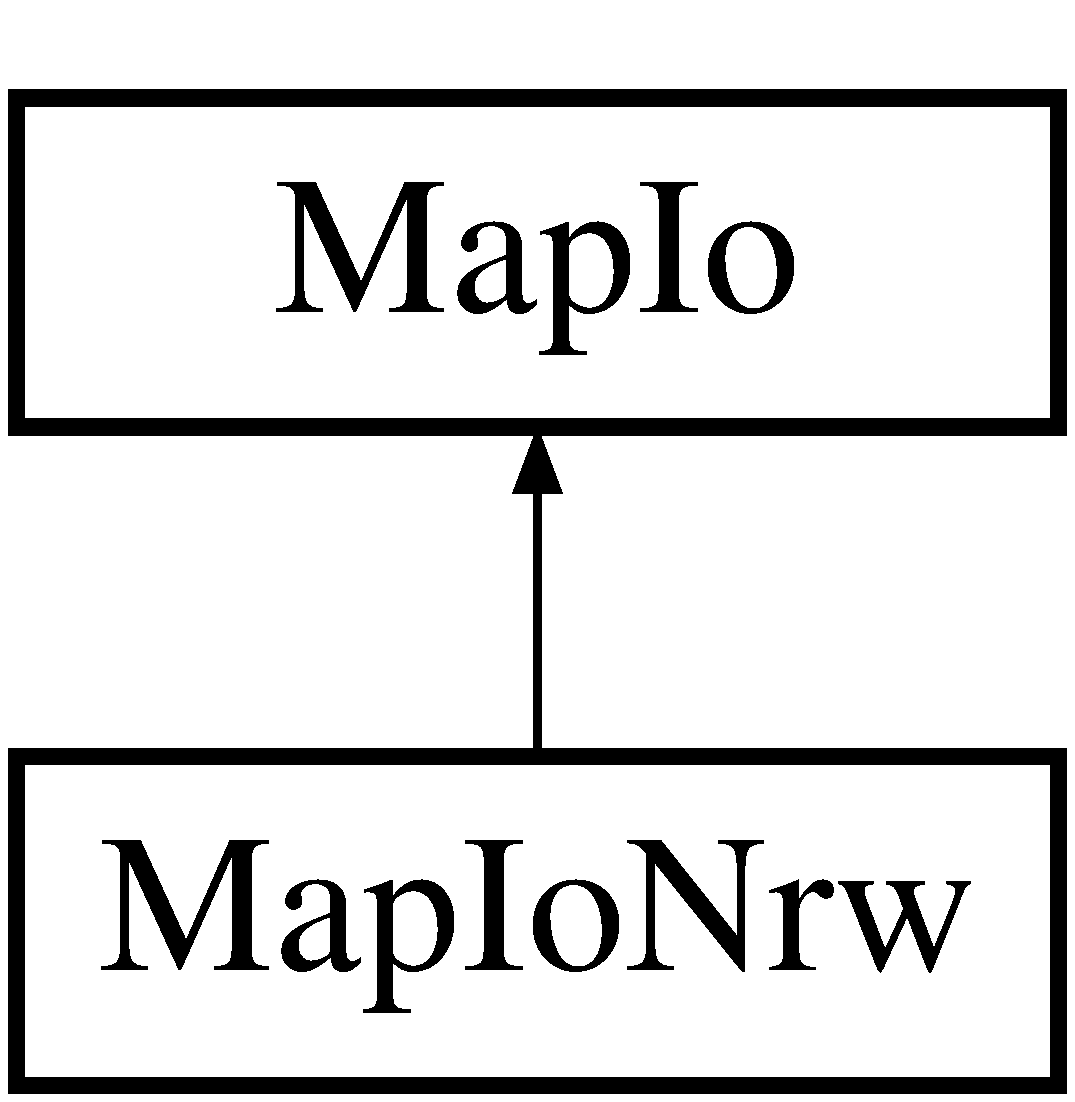
\includegraphics[height=2.000000cm]{class_map_io}
\end{center}
\end{figure}
\subsection*{Public Member Functions}
\begin{DoxyCompactItemize}
\item 
\mbox{\Hypertarget{class_map_io_a72ae6ca54e382dc9cad4b92e92df90c2}\label{class_map_io_a72ae6ca54e382dc9cad4b92e92df90c2}} 
virtual \hyperlink{class_map_io_a72ae6ca54e382dc9cad4b92e92df90c2}{$\sim$\+Map\+Io} ()
\begin{DoxyCompactList}\small\item\em virtual Destructor \end{DoxyCompactList}\item 
\mbox{\Hypertarget{class_map_io_af33256d5aeeb5e36d26660da24bc8ec9}\label{class_map_io_af33256d5aeeb5e36d26660da24bc8ec9}} 
virtual void \hyperlink{class_map_io_af33256d5aeeb5e36d26660da24bc8ec9}{fill\+Map} (\hyperlink{class_abstract_map}{Abstract\+Map} \&map)=0
\begin{DoxyCompactList}\small\item\em this method adds Cities and Streets to the provided \hyperlink{class_map}{Map}. \end{DoxyCompactList}\end{DoxyCompactItemize}


\subsection{Detailed Description}
This class adds Cities and Streeds to a \hyperlink{class_map}{Map}. 

The documentation for this class was generated from the following files\+:\begin{DoxyCompactItemize}
\item 
mapio.\+h\item 
mapio.\+cpp\end{DoxyCompactItemize}

\hypertarget{class_map_io_nrw}{}\section{Map\+Io\+Nrw Class Reference}
\label{class_map_io_nrw}\index{Map\+Io\+Nrw@{Map\+Io\+Nrw}}


This class provides a simple hardcoded \hyperlink{class_map}{Map}.  




{\ttfamily \#include $<$mapionrw.\+h$>$}

Inheritance diagram for Map\+Io\+Nrw\+:\begin{figure}[H]
\begin{center}
\leavevmode
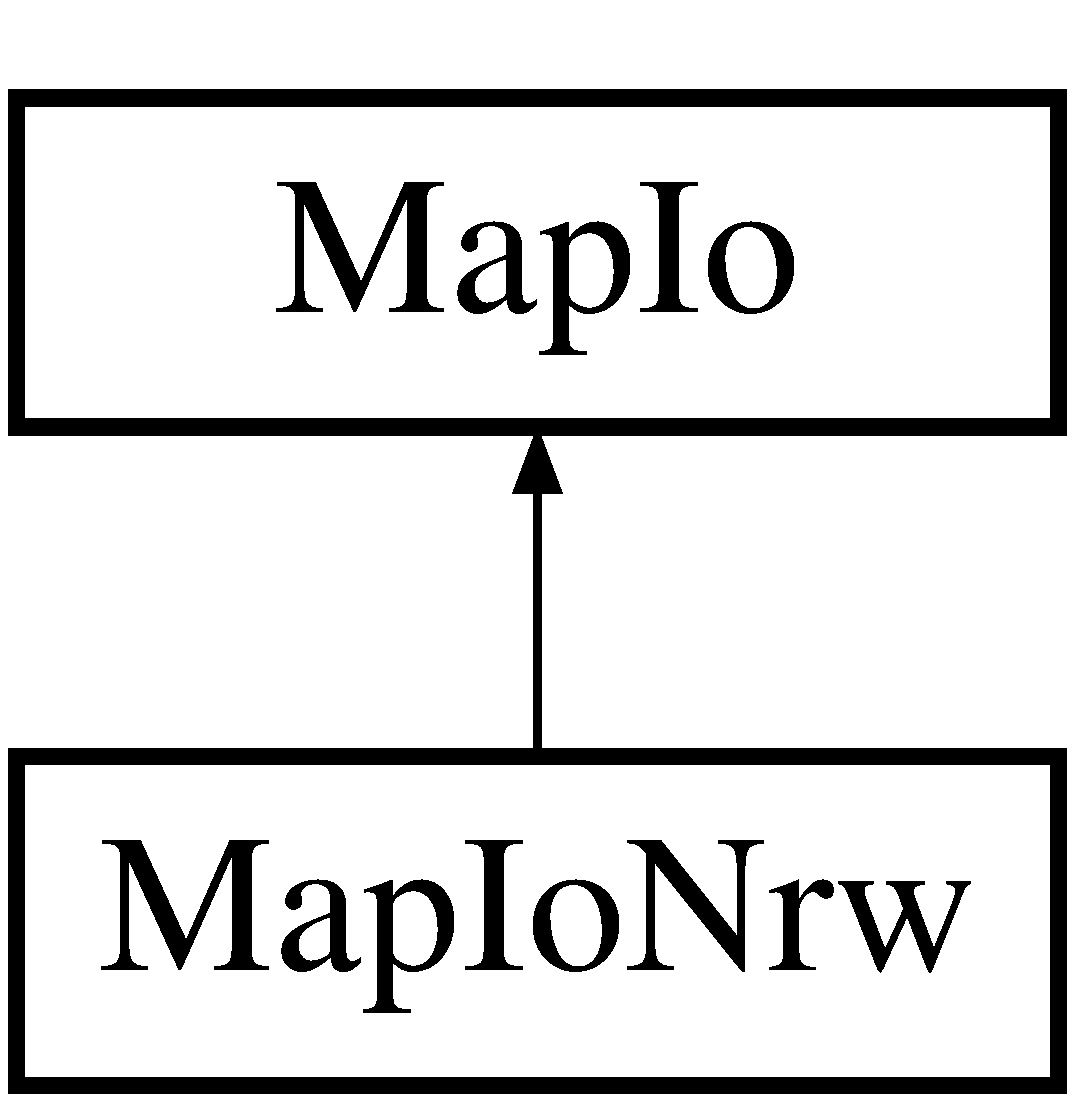
\includegraphics[height=2.000000cm]{class_map_io_nrw}
\end{center}
\end{figure}
\subsection*{Public Member Functions}
\begin{DoxyCompactItemize}
\item 
virtual void \hyperlink{class_map_io_nrw_ab81d348eadcf8f729c3abc6f1e9517e0}{fill\+Map} (\hyperlink{class_abstract_map}{Abstract\+Map} \&map)
\begin{DoxyCompactList}\small\item\em fills a given map with preconfigured cities and streets \end{DoxyCompactList}\end{DoxyCompactItemize}


\subsection{Detailed Description}
This class provides a simple hardcoded \hyperlink{class_map}{Map}. 

\subsection{Member Function Documentation}
\mbox{\Hypertarget{class_map_io_nrw_ab81d348eadcf8f729c3abc6f1e9517e0}\label{class_map_io_nrw_ab81d348eadcf8f729c3abc6f1e9517e0}} 
\index{Map\+Io\+Nrw@{Map\+Io\+Nrw}!fill\+Map@{fill\+Map}}
\index{fill\+Map@{fill\+Map}!Map\+Io\+Nrw@{Map\+Io\+Nrw}}
\subsubsection{\texorpdfstring{fill\+Map()}{fillMap()}}
{\footnotesize\ttfamily void Map\+Io\+Nrw\+::fill\+Map (\begin{DoxyParamCaption}\item[{\hyperlink{class_abstract_map}{Abstract\+Map} \&}]{map }\end{DoxyParamCaption})\hspace{0.3cm}{\ttfamily [virtual]}}



fills a given map with preconfigured cities and streets 


\begin{DoxyParams}{Parameters}
{\em map} & \\
\hline
\end{DoxyParams}


Implements \hyperlink{class_map_io_af33256d5aeeb5e36d26660da24bc8ec9}{Map\+Io}.



The documentation for this class was generated from the following files\+:\begin{DoxyCompactItemize}
\item 
mapionrw.\+h\item 
mapionrw.\+cpp\end{DoxyCompactItemize}

\hypertarget{classnew_city_u_i}{}\section{new\+City\+UI Class Reference}
\label{classnew_city_u_i}\index{new\+City\+UI@{new\+City\+UI}}
Inheritance diagram for new\+City\+UI\+:\begin{figure}[H]
\begin{center}
\leavevmode
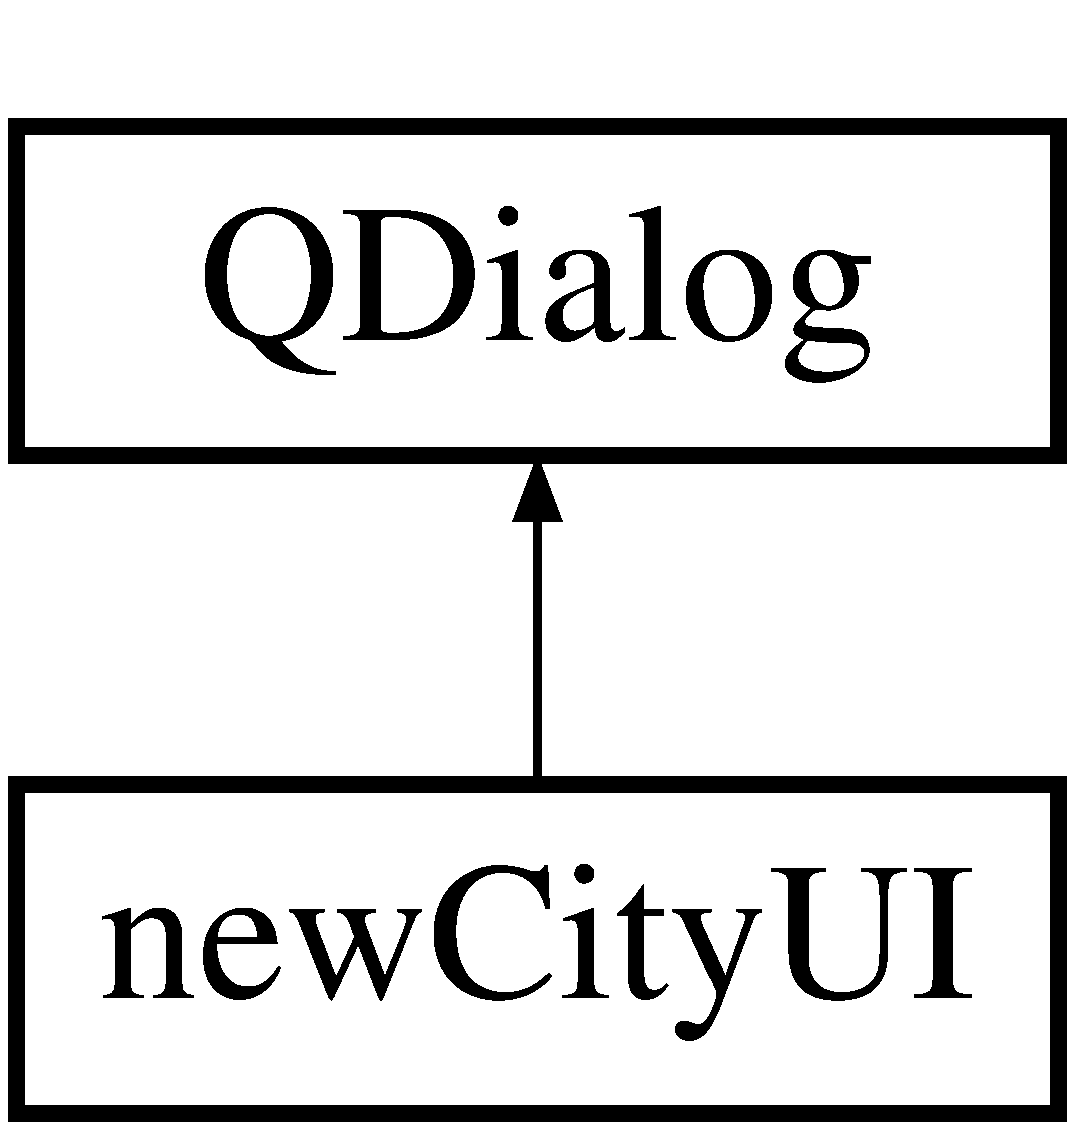
\includegraphics[height=2.000000cm]{classnew_city_u_i}
\end{center}
\end{figure}
\subsection*{Public Member Functions}
\begin{DoxyCompactItemize}
\item 
\mbox{\Hypertarget{classnew_city_u_i_ac4cce3418cc0a4a7b26f471ce5d38da1}\label{classnew_city_u_i_ac4cce3418cc0a4a7b26f471ce5d38da1}} 
{\bfseries new\+City\+UI} (Q\+Widget $\ast$parent=0)
\item 
\hyperlink{class_city}{City} $\ast$ \hyperlink{classnew_city_u_i_ab56f36b8660d9b23280ed3e86927b3c1}{create\+New\+City\+Object} ()
\begin{DoxyCompactList}\small\item\em Returns a new city with the values of the new\+City\+Dialog. \end{DoxyCompactList}\end{DoxyCompactItemize}


\subsection{Member Function Documentation}
\mbox{\Hypertarget{classnew_city_u_i_ab56f36b8660d9b23280ed3e86927b3c1}\label{classnew_city_u_i_ab56f36b8660d9b23280ed3e86927b3c1}} 
\index{new\+City\+UI@{new\+City\+UI}!create\+New\+City\+Object@{create\+New\+City\+Object}}
\index{create\+New\+City\+Object@{create\+New\+City\+Object}!new\+City\+UI@{new\+City\+UI}}
\subsubsection{\texorpdfstring{create\+New\+City\+Object()}{createNewCityObject()}}
{\footnotesize\ttfamily \hyperlink{class_city}{City} $\ast$ new\+City\+U\+I\+::create\+New\+City\+Object (\begin{DoxyParamCaption}{ }\end{DoxyParamCaption})}



Returns a new city with the values of the new\+City\+Dialog. 

\begin{DoxyReturn}{Returns}
The new city 
\end{DoxyReturn}


The documentation for this class was generated from the following files\+:\begin{DoxyCompactItemize}
\item 
newcityui.\+h\item 
newcityui.\+cpp\end{DoxyCompactItemize}

\hypertarget{class_street}{}\section{Street Class Reference}
\label{class_street}\index{Street@{Street}}
\subsection*{Public Member Functions}
\begin{DoxyCompactItemize}
\item 
\mbox{\Hypertarget{class_street_a6b46b32e856030ff31d09ff0011e25e4}\label{class_street_a6b46b32e856030ff31d09ff0011e25e4}} 
{\bfseries Street} (\hyperlink{class_city}{City} $\ast$city1, \hyperlink{class_city}{City} $\ast$city2)
\item 
void \hyperlink{class_street_a8a445d11dfb869969bea3b8f6e4a2edf}{draw} (Q\+Graphics\+Scene \&scene)
\begin{DoxyCompactList}\small\item\em Draws the street between two cities. \end{DoxyCompactList}\item 
\hyperlink{class_city}{City} $\ast$ \hyperlink{class_street_ab8d3699fb6ea3a4da8b1ca9b6b440db8}{get\+City1} () const
\begin{DoxyCompactList}\small\item\em returns city 1 \end{DoxyCompactList}\item 
\hyperlink{class_city}{City} $\ast$ \hyperlink{class_street_af0c8600437fb78a5def8793544970c8c}{get\+City2} () const
\begin{DoxyCompactList}\small\item\em returns city 2 \end{DoxyCompactList}\item 
void \hyperlink{class_street_a64316b1ab76eb572376f47fdb3f8fcc8}{draw\+Red} (Q\+Graphics\+Scene \&scene)
\begin{DoxyCompactList}\small\item\em Draws the street in bold red. \end{DoxyCompactList}\end{DoxyCompactItemize}


\subsection{Member Function Documentation}
\mbox{\Hypertarget{class_street_a8a445d11dfb869969bea3b8f6e4a2edf}\label{class_street_a8a445d11dfb869969bea3b8f6e4a2edf}} 
\index{Street@{Street}!draw@{draw}}
\index{draw@{draw}!Street@{Street}}
\subsubsection{\texorpdfstring{draw()}{draw()}}
{\footnotesize\ttfamily void Street\+::draw (\begin{DoxyParamCaption}\item[{Q\+Graphics\+Scene \&}]{scene }\end{DoxyParamCaption})}



Draws the street between two cities. 


\begin{DoxyParams}{Parameters}
{\em scene} & The Q\+Graphicsscene to draw on \\
\hline
\end{DoxyParams}
\mbox{\Hypertarget{class_street_a64316b1ab76eb572376f47fdb3f8fcc8}\label{class_street_a64316b1ab76eb572376f47fdb3f8fcc8}} 
\index{Street@{Street}!draw\+Red@{draw\+Red}}
\index{draw\+Red@{draw\+Red}!Street@{Street}}
\subsubsection{\texorpdfstring{draw\+Red()}{drawRed()}}
{\footnotesize\ttfamily void Street\+::draw\+Red (\begin{DoxyParamCaption}\item[{Q\+Graphics\+Scene \&}]{scene }\end{DoxyParamCaption})}



Draws the street in bold red. 


\begin{DoxyParams}{Parameters}
{\em scene} & The Q\+Graphicsscene to draw on \\
\hline
\end{DoxyParams}
\mbox{\Hypertarget{class_street_ab8d3699fb6ea3a4da8b1ca9b6b440db8}\label{class_street_ab8d3699fb6ea3a4da8b1ca9b6b440db8}} 
\index{Street@{Street}!get\+City1@{get\+City1}}
\index{get\+City1@{get\+City1}!Street@{Street}}
\subsubsection{\texorpdfstring{get\+City1()}{getCity1()}}
{\footnotesize\ttfamily \hyperlink{class_city}{City} $\ast$ Street\+::get\+City1 (\begin{DoxyParamCaption}{ }\end{DoxyParamCaption}) const}



returns city 1 

\begin{DoxyReturn}{Returns}
city 1 
\end{DoxyReturn}
\mbox{\Hypertarget{class_street_af0c8600437fb78a5def8793544970c8c}\label{class_street_af0c8600437fb78a5def8793544970c8c}} 
\index{Street@{Street}!get\+City2@{get\+City2}}
\index{get\+City2@{get\+City2}!Street@{Street}}
\subsubsection{\texorpdfstring{get\+City2()}{getCity2()}}
{\footnotesize\ttfamily \hyperlink{class_city}{City} $\ast$ Street\+::get\+City2 (\begin{DoxyParamCaption}{ }\end{DoxyParamCaption}) const}



returns city 2 

\begin{DoxyReturn}{Returns}
city 2 
\end{DoxyReturn}


The documentation for this class was generated from the following files\+:\begin{DoxyCompactItemize}
\item 
street.\+h\item 
street.\+cpp\end{DoxyCompactItemize}

\hypertarget{structtuppel}{}\section{tuppel Struct Reference}
\label{structtuppel}\index{tuppel@{tuppel}}
\subsection*{Public Attributes}
\begin{DoxyCompactItemize}
\item 
\mbox{\Hypertarget{structtuppel_aea3598cf38827a307797d8e8ac5549ac}\label{structtuppel_aea3598cf38827a307797d8e8ac5549ac}} 
\hyperlink{class_city}{City} $\ast$ {\bfseries city}
\item 
\mbox{\Hypertarget{structtuppel_a65aa71a1a6b8b896813dfab8222a5b32}\label{structtuppel_a65aa71a1a6b8b896813dfab8222a5b32}} 
double {\bfseries distance}
\item 
\mbox{\Hypertarget{structtuppel_a3cf2fc709ffea8ce66a5dea627365b83}\label{structtuppel_a3cf2fc709ffea8ce66a5dea627365b83}} 
\hyperlink{class_street}{Street} $\ast$ {\bfseries shortest\+\_\+way}
\end{DoxyCompactItemize}


The documentation for this struct was generated from the following file\+:\begin{DoxyCompactItemize}
\item 
dijkstra.\+cpp\end{DoxyCompactItemize}

%--- End generated contents ---

% Index
\backmatter
\newpage
\phantomsection
\clearemptydoublepage
\addcontentsline{toc}{chapter}{Index}
\printindex

\end{document}
